% Pneumatic Braking Mechanism is an implementation of regenerative
% braking mechanism for automobiles. Copyright (C) 2016 Shailendra
% Pratap Verma, Siddharth Singh, Shwetang Dubey and Rishi Anand.

% This work is licensed under the Creative Commons Attribution 4.0
% International License. To view a copy of this license, visit
% http://creativecommons.org/licenses/by/4.0/ or send a letter to
% Creative Commons, PO Box 1866, Mountain View, CA 94042, USA.

\documentclass[12pt,a4paper]{article}

\usepackage{appendix}
\usepackage{amsmath}
\usepackage{amssymb}
\usepackage{enumitem}
\usepackage{float}
\usepackage{graphicx}
\usepackage{nomencl}

\graphicspath{{./images/}}

\makenomenclature
\setlength{\nomitemsep}{-\parsep}

\setlist{noitemsep}

\renewcommand{\nomname}{Appendix A: List of Symbols}
\renewcommand{\listfigurename}{Appendix B: List of Figures}
\renewcommand{\listtablename}{Appendix C: List of Tables}

\title{Pneumatic Braking Mechanism}
\author{Verma, Shailendra Pratap \and Singh, Siddharth \and Dubey, Shwetang \and Anand, Rishi}
\date{May 2016}

\begin{document}

\maketitle

\begin{abstract}
	Pneumatic Braking Mechanism is an implementation of regenerative braking system for automobiles. It uses pneumatic compression to store the kinetic energy of the vehicle. The compressed air is used to produce electricity through a turbine, and then used for supercharging the engine of the automobile.

	The complete mechanism can be divided into two parts:

	\begin{itemize}
		\item Braking
		\item Regeneration
	\end{itemize}

	Regeneration mechanism can be further subdivided into:

	\begin{itemize}
		\item Expansion
		\item Supercharging
	\end{itemize}

	The rotational motion of wheels of the vehicle is used to drive reciprocating compressors. Compressors are engaged with the help of a clutch and crankshaft unit when brakes are applied. Compression process converts the kinetic energy of the vehicle in the form of compressed air. In the process, vehicle loses its energy and comes to a standstill.

	The compressed air goes to a turbine and generator unit where expansion takes place and electricity is produced. The outlet air from turbine at lower pressure is used for supercharging.
\end{abstract}

\section{Introduction}
	Pneumatic Braking Mechanism is a braking mechanism where the kinetic energy of a moving vehicle is conserved in the form of compression work.

	\subsection{Background Work}
		Pneumatic Braking Mechanism is an improvisation of our earlier study on a project titled \emph{Exergy Conservation System — Application of Flywheels}. It is a modification of Flywheel Braking, to obtain better braking performance as well as efficiency.

	\subsection{Regenerative Braking System}
		When an automobile accelerates, chemical energy of the fuel is converted into kinetic energy. In conventional braking, when brakes are applied, the kinetic energy (high grade energy) is dissipated as heat, sound and radiation (low grade energy). In the process, exergy of the vehicle equivalent to its kinetic energy is destroyed. When the vehicle re-accelerates, it again consumes the necessary fuel. The cycle of acceleration/deceleration causes a waste of energy. This creates the need for Regenerative Braking.

		Regenerative Braking System (RBS) captures the energy that is usually lost while braking, stores that energy in an Energy Storage System (ESS) and reuses it to start or accelerate the vehicle.

		An RBS mainly consists of two parts:

		\begin{itemize}
			\item Transmission System
			\item Energy Storage System (ESS)
		\end{itemize}

		Transmission system is used to transmit energy from the wheel to the ESS and vice-versa, while ESS stores the energy. The RBS can be classified on the basis of the ESS. Choice of the transmission is usually dependent and subsequent of the type of ESS selected.

		Types of Energy Storage System (ESS):

		\begin{itemize}
			\item Electro-chemical battery
			\item Ultra-capacitors
			\item Hydraulic and Pneumatic Storage
			\item Mechanical Flywheels
		\end{itemize}

	\subsection{Compressed Air Energy Storage}
		In the compressed air energy storage or pneumatic storage, the energy is stored in form of compressed air. The compression work is a form of high grade energy, and can be readily converted into other forms of energy, theoretically without any losses.

		Advantages:

		\begin{itemize}
			\item Low transmission losses
			\item Low conversion losses
			\item Faster conversion process compared to batteries, capacitors and flywheels thus better braking performance
			\item More robust operation compared to hydraulic storage
		\end{itemize}

	\subsection{Pneumatic Braking Mechanism}
		The Pneumatic Braking Mechanism can be divided into seven parts:

		\begin{description}
			\item [Hydraulic Brake Transmission] The braking transmission is based on the arrangement of hydraulic braking. When the driver pushes the brake pedal, the force is transmitted through the brake fluid, to the callipers at each wheel.
			\item [Clutch and Crankshaft Unit] The clutch and crankshaft unit consists of a friction clutch attached to a crankshaft. When the brake is applied, the clutch is engaged with the rotor disk attached to the wheel, and starts rotating, along with the crankshaft.
			\item [Compressor] A reciprocating compressor, actuated by the rotation of the crankshaft, admits atmospheric air and compresses it.
			\item [Compressed Air Lines] The air from the compressors, travel through the compressed air lines and reach the turbine.
			\item [Turbine and Generator Unit] The turbine and generator unit consists of a two stage axial turbine, attached to a generator shaft, which converts compression work into electrical energy.
			\item [Compressed Air Storage Tank] The air from the turbine unit, is stored in a compressed air storage tank, at a constant pressure.
			\item [Supercharging] The compressed air from the tank is used for supercharging in the IC engine.
		\end{description}

\section{Design Theory}
	\subsection{Clutch and Crankshaft Unit}
		The clutch and crankshaft unit consists of two parts:

		\begin{itemize}
			\item A friction clutch mounted on the crankshaft of reciprocating compressors
			\item A rotor disk attached to the wheels
		\end{itemize}

		\begin{figure}[H]
			\centering
			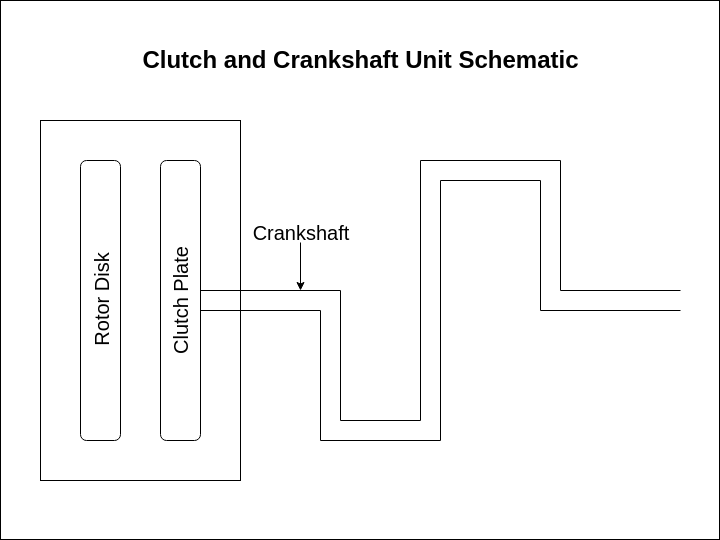
\includegraphics[width=1\textwidth]{images/clutch-and-crankshaft-unit-schematic.png}
			\caption{Clutch and Crankshaft Unit Schematic}
			\label{fig:clutch_and_crankshaft_unit_schematic}
		\end{figure}

	\subsection{Compressor}
		A positive displacement reciprocating type compressor is used to compress air. Atmospheric air is admitted from the surrounding through a suction or inlet valve. The compressed air is expelled from the cylinder through a delivery or outlet valve. The inlet valve operates due to differential pressure while the outlet valve operates due to a spring mechanism.

		\begin{figure}[H]
			\centering
			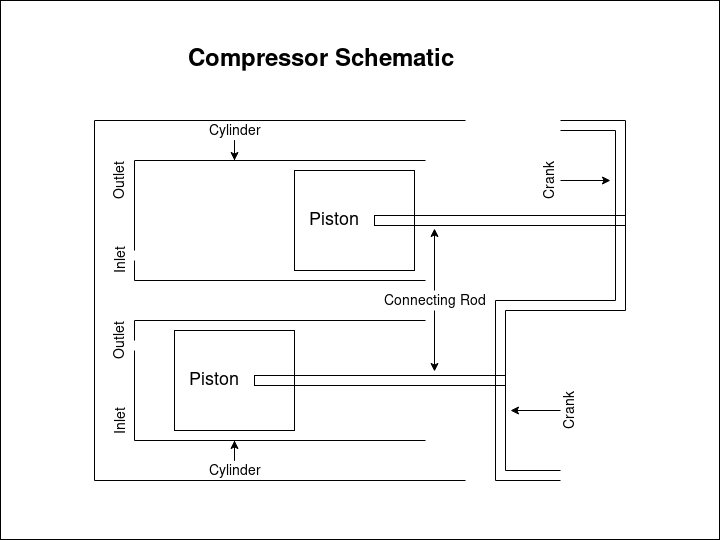
\includegraphics[width=1\textwidth]{images/compressor-schematic.png}
			\caption{Compressor Schematic}
			\label{fig:compressor_schematic}
		\end{figure}

	\subsection{Turbine and Generator Unit}
		The turbine and generator unit consists of a two stage axial turbine coupled with a generator unit.

		\begin{figure}[H]
			\centering
			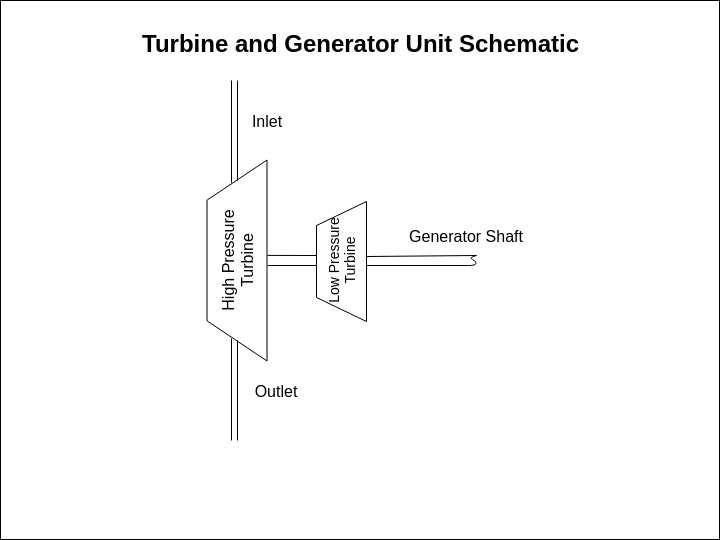
\includegraphics[width=1\textwidth]{images/turbine-and-generator-unit-schematic.png}
			\caption{Turbine and Generator Unit Schematic}
			\label{fig:turbine_and_generator_unit_schematic}
		\end{figure}

\section{Operation Theory}
	The regenerative pneumatic braking is based on conversion of kinetic energy of a moving vehicle into compression work.

	\begin{figure}[H]
		\centering
		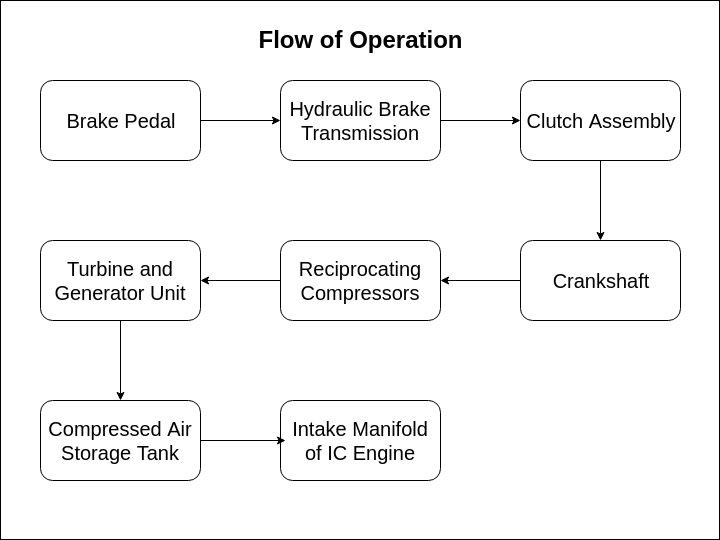
\includegraphics[width=1\textwidth]{images/flow-of-operation.png}
		\caption{Flow of Operation}
		\label{fig:flow_of_operation}
	\end{figure}

	The sequence of processes of the braking mechanism is:

	\begin{enumerate}
		\item Driver pushes the brake pedals to apply the brakes.
		\item The force is transmitted through the hydraulic transmission lines.
		\item At the clutch and crankshaft unit, the fluid pressure due to application of the brakes engages the clutch and rotor disk.
		\item The crankshaft attached to the clutch starts rotating due to the motion of wheels.
		\item The brake pedal causes a push-rod to exert force on the primary piston present in the master cylinder.
		\item The crankshaft converts the rotary motion of the wheel into the reciprocating motion of the piston of the compressor.
		\item The compressor admits air at atmospheric pressure, and compresses it.
		\item When the pressure inside the compressor reaches a predetermined maximum, the outlet valve opens.
		\item The compressed air from the reciprocating compressor travels to the turbine and generator unit where it undergoes expansion.
		\item The turbine converts the compression work into electrical energy.
		\item The air from the turbine goes to the intake manifold of the IC engine, where it is used for supercharging.
	\end{enumerate}

	\subsection{Clutch and Crankshaft Unit}
		The clutch is operated by the hydraulic braking transmission. When the brakes are applied, the pressure causes the clutch to engage with the rotor disks, and the pair starts rotating due to friction.

		The crankshaft is attached to the clutch. The crank is connected to the piston of the reciprocating compressors using connecting rod.

	\subsection{Compressor}
		\begin{figure}[H]
			\centering
			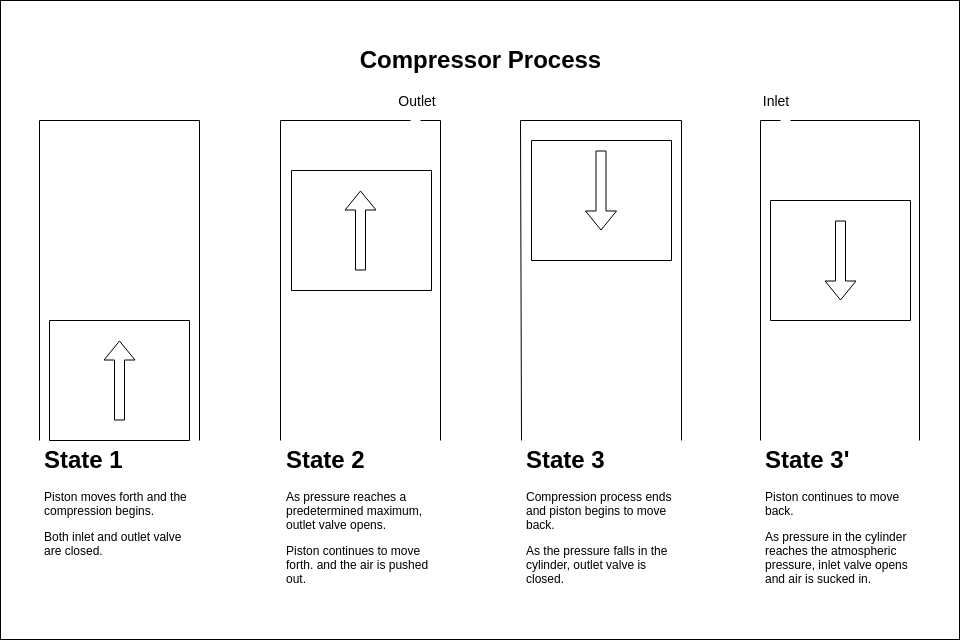
\includegraphics[width=1\textwidth]{images/compression-process.png}
			\caption{Compression Process}
			\label{fig:compression_process}
		\end{figure}

		The compression of air in the double reciprocating compressor is a sequence of four processes:

		\begin{enumerate}
			\item Air in the cylinder at atmospheric pressure undergoes adiabatic compression.
			\item As the air reaches the predetermined maximum pressure, the outlet valve of the cylinder opens. Compressed air is pushed out, while the piston continues to compress the remaining air at constant pressure.
			\item As the compression process ends, and the piston starts moving out. As the air pressure inside the cylinder drops, the outlet valve closes, and the air expands at constant volume.
			\item As the piston continues to move back, atmospheric air is sucked into the cylinder through the inlet port.
		\end{enumerate}

	\subsection{Turbine and Generator Unit}
		The air from the all the compressors travels through the compressed air lines and reaches the turbine and generator unit. Air enters the high pressure turbine where it undergoes adiabatic expansion. The expanded air then goes to the low pressure turbine where it undergoes further expansion up to a pressure suitable for supercharging. The generator unit converts the mechanical energy from the turbine into electrical energy.

\section{Numerical Theory}
	\subsection{Assumptions} \label{sec:numerical_theory_assumptions}
		For numerical calculations, the following values are assumed

		\begin{table}[H]
			\centering
			\begin{tabular}{r r}
				Quantity & Value \\
				\( \gamma \) & 1.4 \\
				\( p_1 \) & 1 bar \\
				\( p_2 \) & 10 bar \\
				\( k \) & 8 \\
				\( d \) & 20 cm \\
				\( L \) & 30 cm \\
				\( M \) & 1000 kg \\
				\( D \) & 0.5 m
			\end{tabular}
			\caption{Assumptions}
			\label{tab:assumed_values}
		\end{table}

	\subsection{Compression Process}
		\begin{figure}[H]
			\centering
			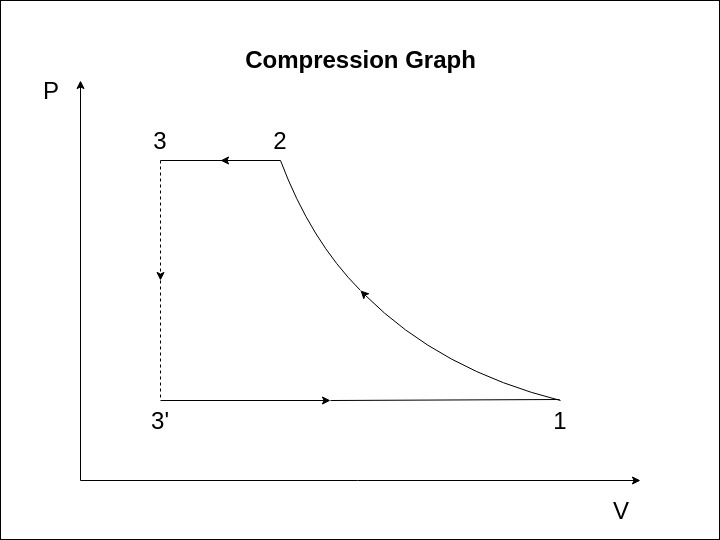
\includegraphics[width=1\textwidth]{images/compression-graph.png}
			\caption{Compression Graph}
			\label{fig:compression_graph}
		\end{figure}

		The compression of air is a sequence of four processes:

		\begin{description}
			\item[Process 1 - 2] Adiabatic Compression
			\item[Process 2 - 3] Isobaric Compression
			\item[Process 3 - 3'] Isochoric Expansion
			\item[Process 3' - 1] Isobaric Expansion
		\end{description}

		Compression Work on the air in one revolution,

		\begin{align*}
			W &= W_{1-2} + W_{2-3} - W_{3'-1} \\
			  &= \frac{p_2 V_2 - p_1 V_1}{\gamma - 1} + p_2 (V_2 - V_3) - p_1 (V_1 - V_{3'})
		\end{align*}

		\nomenclature[00]{\( \gamma \)}{Adiabatic Constant}
		\nomenclature[01]{\( W \)}{Compression work in one cycle}
		\nomenclature[02]{\( W_{1-2} \)}{Work done during adiabatic compression}
		\nomenclature[03]{\( W_{2-3} \)}{Work done during isobaric compression}
		\nomenclature[04]{\( W_{3'-1} \)}{Work lost during isobaric expansion}
		\nomenclature[05]{\( p_1 \)}{Inlet pressure of compressor}
		\nomenclature[06]{\( p_2 \)}{Outlet pressure of compressor}
		\nomenclature[07]{\( V_1 \)}{Volume of the cylinder before compressor begins}
		\nomenclature[08]{\( V_2 \)}{Volume of the cylinder when outlet valve opens}
		\nomenclature[09]{\( V_3 \)}{Volume of the cylinder when the compression ends}
		\nomenclature[10]{\( V_{3'} \)}{Volume of the cylinder when inlet valve opens}

		Considering only adiabatic Work,

		\begin{equation} \label{eq:compression_work}
			\boxed{W = \frac{p_2 V_2 - p_1 V_1}{\gamma - 1}}
		\end{equation}

		Net work in one revolution,

		\begin{equation*}
			W_{NET} = k \times W
		\end{equation*}

		\begin{equation} \label{eq:net_work}
			\implies \boxed{W_{NET} = k \times \frac{p_2 V_2 - p_1 V_1}{\gamma - 1}}
		\end{equation}

		\begin{equation*}
			\implies W_{NET} = k \times \frac{p_1 V_1}{\gamma - 1} \times \left[1 - \left(\frac{p_2}{p_1} \right) ^ \frac{\gamma - 1}{\gamma} \right]
		\end{equation*}

		\nomenclature[11]{\( W_{NET} \)}{Net work by all the compressors in one revolution}
		\nomenclature[12]{\( k \)}{Total number of the compressors}

		Pressure \( p_1 \), Volume \( V_1 \) are constant for the process, due to constant atmospheric pressure and cylinder volume.

		\begin{equation} \label{eq:net_work_vs_outlet_pressure}
			\therefore \boxed{W_{NET} \propto k \left[1 - c_1 \times p_2 ^ \frac{\gamma - 1}{\gamma} \right]}
		\end{equation}

		\begin{equation*}
			\text{where,} c_1 = \frac{1}{p_1 ^ \frac{\gamma - 1}{\gamma}}
		\end{equation*}

		Using equation~\ref{eq:net_work_vs_outlet_pressure} and the values from section~\ref{sec:numerical_theory_assumptions}, the graph of Net Compression Work vs Outlet Pressure can be obtained as,

		\begin{figure}[H]
			\centering
			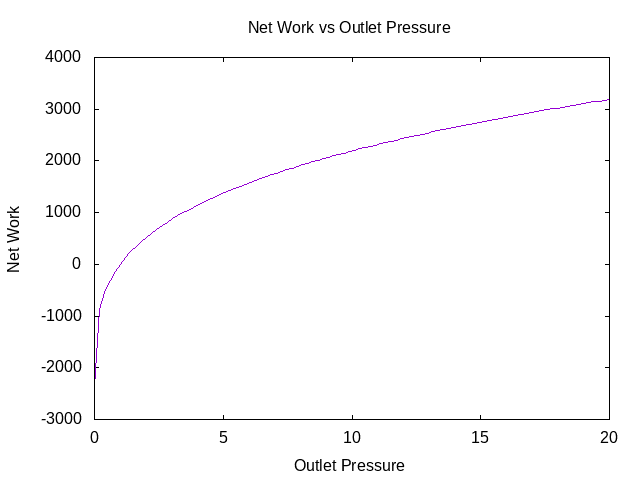
\includegraphics[width=1\textwidth]{images/work-vs-pressure.png}
			\caption{Net Work vs Outlet Pressure}
			\label{fig:net_work_vs_outlet_pressure}
		\end{figure}

		The following observations can be made from the graph:

		\begin{itemize}
			\item The work done increases with the increase in outlet pressure.
			\item The slope of curve decreases with increase in outlet pressure.
		\end{itemize}

		Volume of the air in the cylinder before compression begins,

		\begin{equation*}
			V_1 = \frac{\pi}{4} \times d^2 \times L = 9.4247 \times 10^{-3} \ m^3
		\end{equation*}

		\nomenclature[13]{\( d \)}{Bore diameter of the cylinder}
		\nomenclature[14]{\( L \)}{Length of the cylinder}

		For adiabatic compression process,

		\begin{equation*}
			\frac{p_2}{p_1} = \left(\frac{V_1}{V_2} \right) ^ \gamma
		\end{equation*}

		Volume of air in the cylinder at the end of adiabatic compression,

		\begin{equation*}
			\implies V_2 = 1.8196 \times 10^{-3} \ m^3
		\end{equation*}

		Substituting the values of \( p_1, \ p_2, \ V_1, \ V_2 \) and \( k \) in equation~\ref{eq:net_work},

		\begin{equation*}
			\boxed{W_{NET} = 17542.6 \ J}
		\end{equation*}

	\subsection{Kinetic Energy Analysis}
		Kinetic Energy of the vehicle,

		\begin{equation} \label{eq:kinetic_energy}
			KE = \frac{1}{2} \times M \times v^2 = 500 \times v^2
		\end{equation}

		\nomenclature[15]{\( M \)}{Mass of the vehicle}
		\nomenclature[16]{\( v \)}{Speed of the vehicle}
		\nomenclature[17]{\( KE \)}{Kinetic Energy of the vehicle}

		For the vehicle to come to standstill, its kinetic energy must get transformed into the energy of compressed air.

		Number of rotations of the wheel before the vehicle comes to standstill,

		\begin{align*} \label{eq:no_of_rotations}
			n &= \frac{KE}{W_{NET}} \\
			  &= \frac{500 \times v^2}{17542.6} \ rotations
		\end{align*}

		\nomenclature[18]{\( n \)}{Number of rotations of wheels before the vehicle stops}

		Stopping Distance,

		\begin{align*}
			\Delta x &= n \times \pi \times D \\
					 &= \frac{500 \times v^2}{17542.6} \times \pi \times 0.5
		\end{align*}

		\begin{equation} \label{eq:stopping_distance}
			\boxed{\Delta x = 0.0448 \times v^2 \ m}
		\end{equation}

		\nomenclature[19]{\( D \)}{Diameter of the wheels of the vehicle}
		\nomenclature[20]{\( \Delta x \)}{Stopping distance}

\section{Conclusions}
	\subsection{Stopping Distance Calculations}
		Using equation~\ref{eq:stopping_distance}, stopping distance for various speeds can be obtained

		\begin{table}[H]
			\centering
			\begin{tabular}{r r}
				Speed of the vehicle, \( v \ (kmph) \) & Stopping distance, \( \Delta x \ (m) \) \\
				20 & 1.3827 \\
				50 & 8.6420 \\
				100 & 34.5679
			\end{tabular}
			\caption{Stopping Distances}
			\label{tab:stopping_distances}
		\end{table}

\begin{thebibliography}{9}
	\bibitem{regenerative_brakes}
		Woodford, Chris. (2009/2018) Regenerative brakes. Retrieved from https://www.explainthatstuff.com/how-regenerative-brakes-work.html. [Accessed 2 November, 2018]
	\bibitem{regenerative_system}
		Kubierschky, Martin TA. "Regenerative system." U.S. Patent 714,196, issued November 25, 1902.
	\bibitem{fluid_pressure_braking_system}
		Bishop, Boughton Edward, Emmott Willie, and Brock Denis Tabor. "Fluid pressure braking system." U.S. Patent 2,008,975, issued July 23, 1935.
	\bibitem{regenerative_energy_transfer_system}
		Taylor, Heyward T., and Michael B. Lambert. "Regenerative energy transfer system." U.S. Patent 4,348,863, issued September 14, 1982.
	\bibitem{regenerative_compression_braking}
		Schechter, Michael M. "Regenerative Compression Braking―A Low Cost Alternative to Electric Hybrids." \textit{SAE Transactions} 109 (2000): 1192-203. http://www.jstor.org/stable/44634298.
	\bibitem{analysis_of_compressed_air_regenerative_braking}
		Wicks, Frank, Justin Maleszweski, Colin Wright, and Jan Zarybnicky. "Analysis of compressed air regenerative braking and a thermally enhanced option." \textit{In Energy Conversion Engineering Conference, 2002. IECEC'02. 2002 37th Intersociety}, pp. 406-411. IEEE, 2004.
	\bibitem{pneumatic_hybrid_vehicle}
		Trajkovic, Sasa. \textit{The Pneumatic Hybrid Vehicle-A New Concept for Fuel Consumption Reduction}. Lund University, 2010.
	\bibitem{power_generation_directly_from_compressed_air}
		Gerard, Henry M. "Power generation directly from compressed air for exploiting wind and solar power." U.S. Patent 8,347,628, issued January 8, 2013.
	\bibitem{internal_combustion_engines_supercharging}
		Ganesan, V. "Supercharging." \textit{Internal combustion engines}, 597-610. McGraw Hill Education (India) Pvt Ltd, 2012.
\end{thebibliography}

\begin{appendices}
	\printnomenclature{}
	\listoffigures
	\listoftables
\end{appendices}
\end{document}
